\documentclass[xcolor={usenames,dvipsnames},aspectratio=169, 12pt]{beamer}
\usetheme[color={default},hideothersubsections]{UH-Slides-ECE}
\titleimage{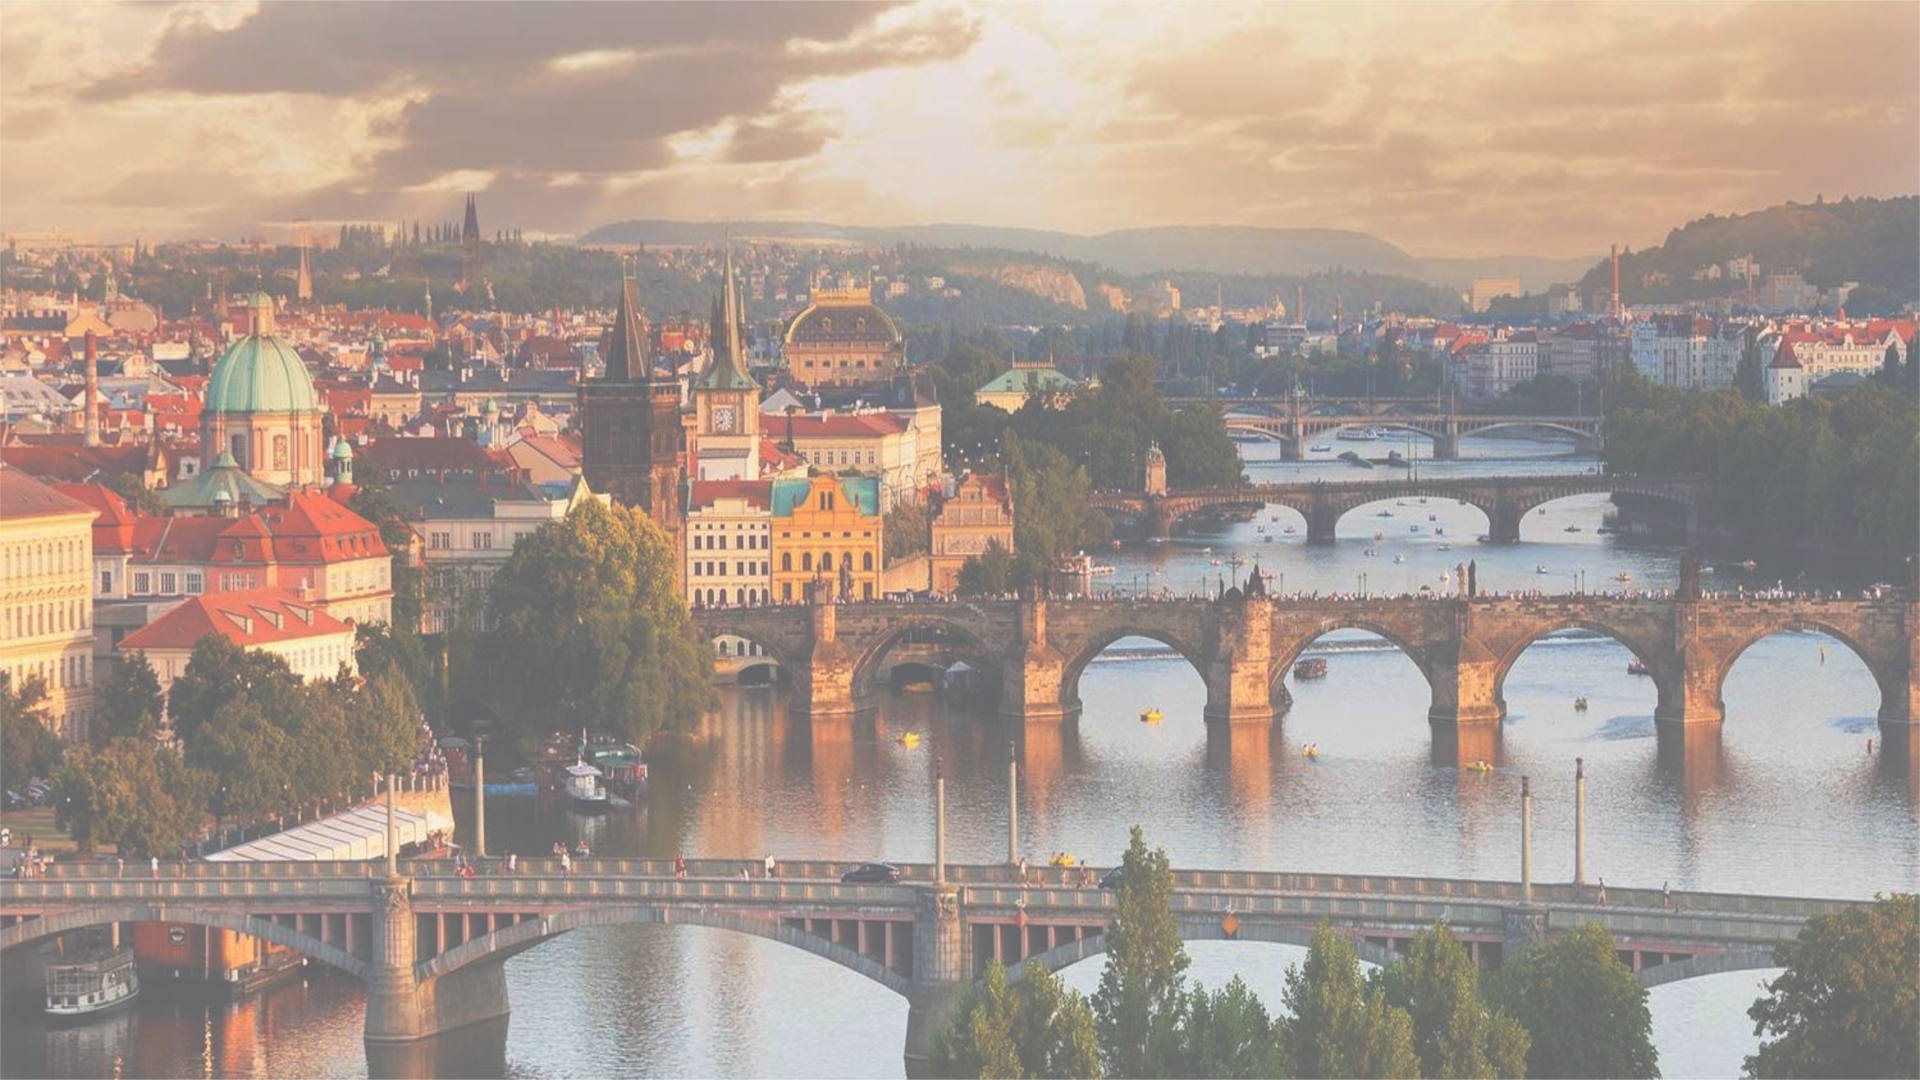
\includegraphics[width=\paperwidth]{assets/praha_title.png}} % SET YOUR BACKGROUND IMAGE HERE FOR THE TITLE
\hypersetup{
    colorlinks=true, % Enables coloring of links
    linkcolor=blue,  % Color for internal links
    filecolor=magenta, % Color for URLs which open local files
    urlcolor=blue,   % Color for linked URLs
    citecolor=green   % Color for bibliographic citations in text
}

% Uncomment this to use serif font
\usefonttheme{serif} % Use serif font theme

%\setbeameroption{show notes} % Use this command to produce notes for slides.

\title{Insert TIitle Here}
\author{Your Name}
\subtitle{You can put a subtitle here}
\institute{Charles University}



% This will be displayed at the beginning of each section delete it if you dont want outline to be there all the time
\AtBeginSection[] {
\begin{frame}
  \frametitle{Outline}
  \tableofcontents[currentsection]
\end{frame}
}

\date[\MONTH~\the\day] % appears in the bottom of the sidebar
{\today}

\begin{document}

\titleframe

\section{Introduction}
\subsection{Overview}
\begin{frame}
\frametitle{Intro}
  \begin{itemize}
    \item<1-> This works as classical beamer presentation
    \begin{itemize}
      \item<2-> \textbf{Displaying stuff}
      \begin{itemize}
        \item<2-> As you can see the next to be displayed text is dimmer
      \end{itemize}
      \item<3-> \textbf{Transitions}
      \begin{itemize}
        \item<3-> The subsub items are not displayed until the next slide
      \end{itemize}
      \item<4-> \textbf{Random text}
      \begin{itemize}
        \item<4-> Lorem Ipsum
      \end{itemize}
    \end{itemize}
  \end{itemize}
\end{frame}

\subsection{Motivation}
\begin{frame}
\frametitle{Why use this}
\begin{itemize}
  \item Looks cool
\end{itemize}
\begin{itemize}
  \item I don't know what more
\end{itemize}
\begin{block}{Display of math looks nice}
  \begin{equation}
    \sum_{i=1}^{n} i = \frac{n(n+1)}{2}
  \end{equation}
\end{block}
You can cite here classicly using \texttt{cite} command. For example \cite{lapointe1997average}.
\end{frame}

\section{The End}
\subsection{Figures}
\begin{frame}
\frametitle{Displaying figures}
  \begin{figure}[htbp]
    \centering
    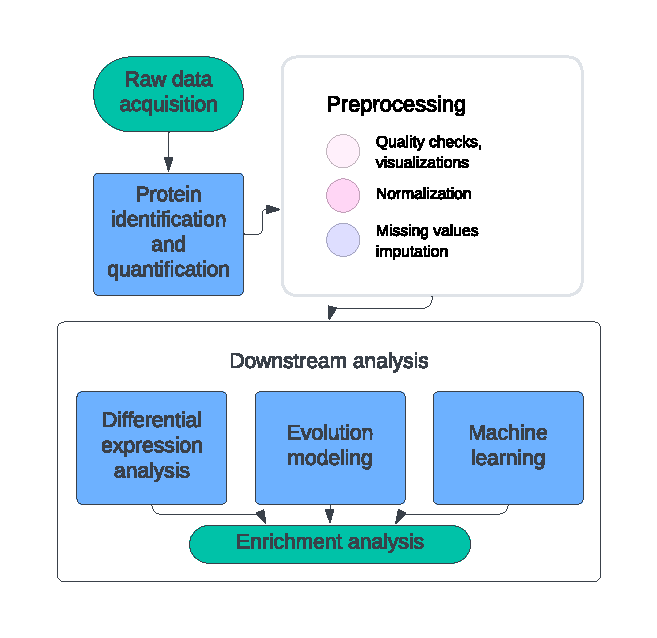
\includegraphics[width = 0.45\textwidth]{assets/proposed_pipeline2.pdf}
    \caption{Pipeline I used in my bachelors thesis.}
    \DeclareGraphicsExtensions.
  \end{figure}
\end{frame}


\section{References}
%
\begin{frame}[allowframebreaks]
\frametitle{Reference}
\footnotesize
\bibliographystyle{IEEEtran}
% argument is your BibTeX string definitions and bibliography database(s)
\bibliography{bib/ref_nn}
\end{frame}

\ThankYouFrame

\end{document}